

\subsection{\em Dataset}
We've constructed synthetic data to manually make temporally changing points. A tensor has its size of $10*20*30*1000$ having the last mode as a temporal mode. The tensor $\chi$ was conducted by concatenation of theme tensor $T$ which is addition of three tensors $T_{main}$, $T_{theme}$ and $T_{noise}$. Each consisting tensor is 100x, 10x and 1x normal distributed randomized tensor respectively and those are used for making different and similar theme tensors.

\begin{table}[htb]
\small
\begin{tabular}{ c | cccccccccc }
 \hline
 Time Index & 1$\sim$100 & 101$\sim$200 & 201$\sim$250 & 251$\sim$500 & 501$\sim$600 & 601$\sim$700 & 701$\sim$750 & 751$\sim$800 & 801$\sim$950 & 951$\sim$1000 \\
 \hline
 Theme & $A$ & $A'$ & $B$ & $B'$ & $B''$ & $C$ & $D$ & $E$ & $E'$ & $E''$ \\
 \hline
\end{tabular}
\end{table}

\subsection{\em Experimental Setting}
In the experiment, we've set rank as 10, temporal batch size as 1 and initial size for \ocp as 5.
 
\begin{center}
	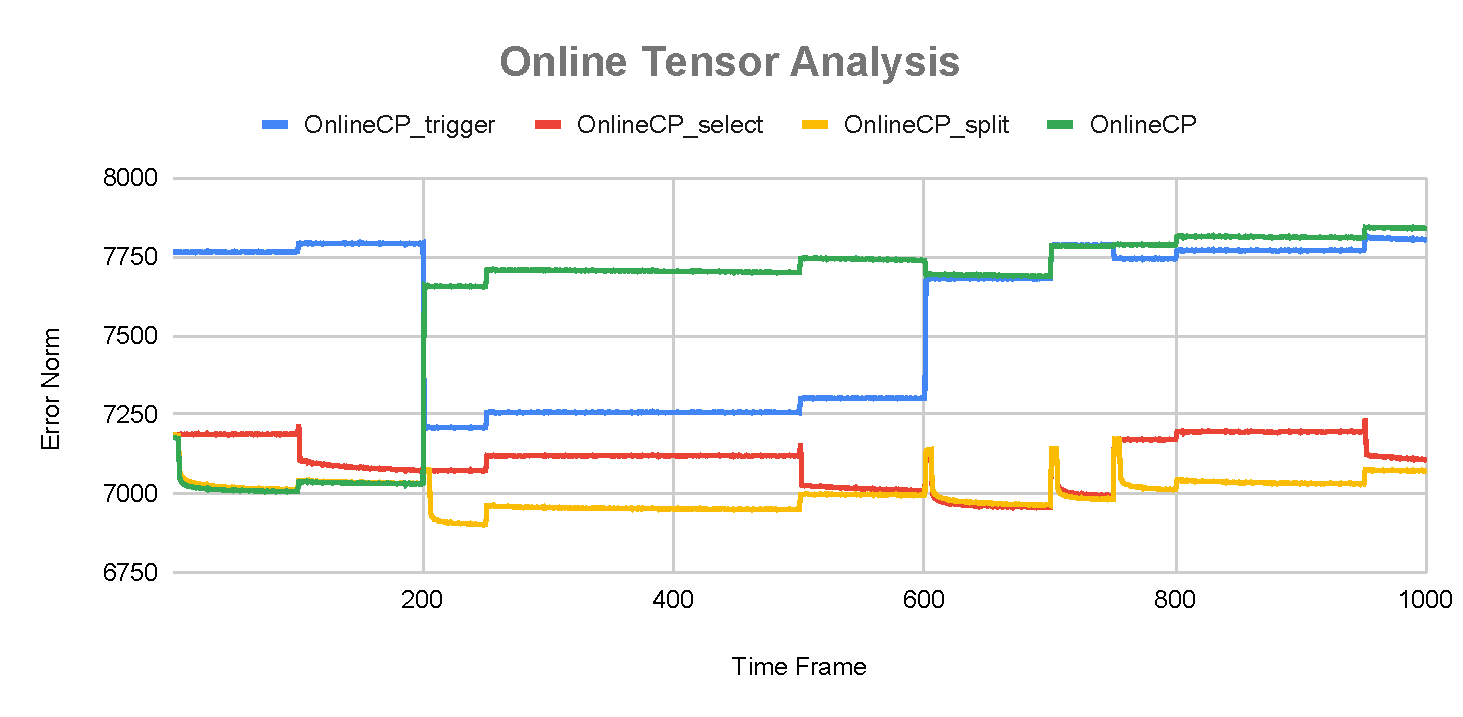
\includegraphics[width=1\textwidth]{FIG/Comparison-analysis.pdf}
\end{center}
